\documentclass[conference]{IEEEtran}
% \IEEEoverridecommandlockouts
% The preceding line is only needed to identify funding in the first footnote. If that is unneeded, please comment it out.
\usepackage{cite}
\usepackage{amsmath,amssymb,amsfonts}
\usepackage{algorithmic}
\usepackage{graphicx}
\usepackage{textcomp}
\usepackage{xcolor}
\usepackage{hyperref}
\usepackage{subfig}
\usepackage[font=scriptsize]{caption}
\def\BibTeX{{\rm B\kern-.05em{\sc i\kern-.025em b}\kern-.08em
    T\kern-.1667em\lower.7ex\hbox{E}\kern-.125emX}}

\newcommand\ci{\perp\!\!\!\perp}

\begin{document}

\title{Noninvasive Discovery of Network Traffic Patterns\\
}
\author{\IEEEauthorblockN{Clara Cousins}
\IEEEauthorblockA{\href{mailto:ccousins@college.harvard.edu}{ccousins@college.harvard.edu}}
\and
\IEEEauthorblockN{William Drew}
\IEEEauthorblockA{\href{mailto:wdrew@college.harvard.edu}{wdrew@college.harvard.edu}}
}
\maketitle
\begin{abstract}
Despite needing to identify the origins of their own and others' internet traffic, competing content service providers may not have access to packet-level information at each others' servers. We propose a novel, noninvasive solution to identify network-wide traffic flows using only packet counts at internet service provider routers by learning directed acyclic graphs (DAGs). We use simulated data in multiple topologies and identify the fast incremental association Markov blanket (IAMB) algorithm as an appropriate structure learning algorithm. For networks with tree and mesh components, we found that the ratio of true found edges to total true edges is 0.76, while the ratio of falsely found edges to total found edges is 0.39, indicating that DAG structure learning may be suitable for revealing network-wide traffic flows.

\end{abstract}

\begin{IEEEkeywords}
internet, topology, flow, network, noninvasive
\end{IEEEkeywords}

\section{Introduction}
With an increasing reliance on internet networks to deliver content to consumers, there is a growing need for network analysis tools that enable businesses to understand their own network traffic footprint and that of their competitors. However, due to the sensitivity of network traffic information including port number, protocol type, and packet routing path, there is also a challenging demand to recover network traffic flows from information that is not embedded in the packets themselves.  A noninvasive network analysis method would be revolutionary to the field. In this work, we explore how directed acyclic graphs (DAGs) can represent network traffic flows across hosts using only packet count statistics at routers.

\section{Problem to Solve}

This project asks: To what extent does DAG structure learning reveal computer network traffic flows based on router packet counts?

\section{Background, Motivations, and Prior Work}

Content delivery services, such as Netflix and Hulu, compete for consumers but may not have access to read the packets at each other's routers or servers. Netflix and Hulu would be motivated to compare their traffic flow patterns among a collection of routers (such as for a certain internet service provider in the metro Boston area) in order to identify the routers that are bottlenecks for their network traffic as well as the geographical areas or parts of the network that each company reaches effectively \cite{b1}.

Many techniques are currently used to identify traffic at various degrees of granularity, including the packet, individual host, or aggregate host (i.e., local area network [LAN]) levels. At the packet level, packet header information may be required to determine the source and destination addresses and ports. One such example of network traffic monitoring at the packet level is implemented in Cisco NetFlow \cite{b2}. Cisco NetFlow is an arguably invasive approach to analyzing network traffic as it requires packet header inspection using NetFlow-enabled devices. At the individual host level, network traffic can be understood for a given router by probing networks with dummy packets, but this method does not scale well to collections of hosts since they increase traffic and may resemble distributed denial of service attacks \cite{b3}. Across hosts, graphical models have been used to summarize traffic flows. Traffic dispersion graphs (TDGs), used by \cite{b1}, treat IP addresses as nodes and use directed edges to represent node-interactions (i.e., traffic among hosts) over a given time interval. TDGs for HTTP traffic may be derived by inspecting the port number of certain packets, such as TCP SYN packets, and setting an edge between the source and destination hosts for that packet if port 80 is used at the destination \cite{b1}. The topology of the TDG provides a useful representation of traffic aggregated at the host level.

We aim to solve the problem of how to represent network traffic in a local area network (LAN) at the level of aggregate host flows without using invasive route traces involving the specific servers of interest. Solving this problem would be useful for competitors seeking to understand traffic flow patterns in a LAN in order to detect bottlenecks and regions of particularly high usage even if the available data is simply packet count at routers in the LAN. This could enable content service providers to craft new subscriber services, optimize shared resource utilization, and understand the limitations of the content delivery network.


\section{Project Goals \& Evaluation Metric}

The goal of this project is to determine with DAG structure learning algorithms can reveal accurate traffic flow topologies using simulated networks adhering to a link state routing scheme using Dijkstra's shortest path algorithm. This goal would be successfully achieved if
\[
\frac{\text{True DAG edges}}{\text{Total edges in ground truth topology}} > \frac{\text{False DAG edges}}{\text{Total edges in DAG}}
\]

\section{Proposed Approach, Novelty and Secret Weapon}

We propose a novel method to learn aggregate flows across hosts using only packet counts at routers. Critically, this approach noninvasively learns network traffic flows without examining sensitive fields such as destination IP addresses, port numbers, protocol types, and other information that can be collected from data packet headers. We accomplish this using DAG structure learning algorithms to predict network traffic flows.

\section{Intellectual Points}

Directed acyclic graphs (DAGs) encode the joint probability distribution of a collection of random variables ("nodes”) without allowing conditional dependencies ("edges”), interpreted as directed causal effects, to form cycles among the nodes. Conditional independence exists between random variables $X$ and $Y$ given $Z$ with nonzero probability $\left(X \ci Y | Z \right)$ if $P(X \ci Y | Z) = P(X | Z) * P(Y | Z)$ where $P(A | B) = P(A, B) / P(B)$. Because DAGs are probabilistic graphical models, they provide statistical power to detect the true conditional dependencies but ultimately rely on certain assumptions to allow causality to be inferred. Three major assumptions of DAGs include the causal Markov condition, faithfulness, and causal sufficiency \cite{b4}. Briefly, the causal Markov condition, which allows edges to be interpreted as causal effects, states that a node is conditionally independent of all other nodes except for its children (direct descendants) given its parents (direct causes of the node)\cite{b5}. Faithfulness means that the DAG learned from the data contains conditional dependencies that are indeed reflected in the data and are not the result of model parameters cancelling each other during the learning process \cite{b6}. Finally, causal sufficiency ensures that enough nodes are included in the DAG such that the conditional dependencies learned have the potential to reflect real causal effects without hidden nodes being responsible for the relations \cite{b6}.

In order to model network traffic flows on the aggregate host level because even if cycles exist, we are not interested in learning them because we primarily want to find sources versus destinations so want to constrain flows not to be starting and ending at the same host in a cyclic flow. Note that even though we expect most flows not to contain cycles, we still test to see if a DAG models real traffic flows in real networking data since we could a dataset that does provide routes so we can check which links are recapitulated in the learned DAG.

There are three main classes of algorithms used to learn the structure of a DAG from observational data (i.e., without manipulation of the values at any node). Briefly, score-based approaches (such as greedy hill-climbing) begin with a random DAG structure and scores it on goodness-of-fit relative to the data, then makes every possible perturbation (either adding, removing, or reversing direction of an arc) to the DAG, rescores the fit, then updates the DAG (making the perturbation that will maximize the score from the given space in the search) structure in order to maximize the score, stopping once perturbations no longer exist that improve the score \cite{b7}. Various scores may be used in hill-climbing, including the log-likelihood, Bayesian Information Criterion (BIC), and Akaike's Information Criterion (AIC), with the latter two being regularized versions of log-likelihood.

Constraint-based algorithms, such as the PC ("Peter and Clark") algorithm \cite{b8}, identify directed edges in the DAG by conditional independence testing. Specifically, constraint-based algorithms begin with saturated DAGs (having every possible causal relation indicated) and eliminate arcs according to the conditional independence relations in the data \cite{b7}. Different conditional independence tests exist, including \href{http://www.bnlearn.com/documentation/man/conditional.independence.tests.html}{Pearson's linear correlation test with Student's t}.

The incremental association Markov blanket (IAMB) algorithm is another constraint-based algorithm \cite{b9} that relies on conditional independence testing to eliminate edges from the saturated Markov blanket for each node (i.e., the node's parents, node's children, and other parents of the node's children) as opposed to the entire saturated undirected graph in the PC algorithm.

Hybrid algorithms use conditional independence testing to build initial DAGs from which score-based approaches can search from this restricted space to determine a DAG that fits the data well \cite{b7}. One hybrid algorithm is the  \href{https://link.springer.com/article/10.1007/s10994-006-6889-7}{Max-Min Hill-Climbing algorithm}, which constructs the DAG skeleton by the PC algorithm and then uses this as the initial DAG from which the hill-climbing algorithm can be used to search a reduced search space to direct the edges.

The algorithms have different accuracies for different topologies, but the conditions for which each algorithm performs best are not well understood \cite{b10}. Which algorithm may learn computer network traffic flow patterns best for different topologies is not known. In order to learn aggregate flows across hosts and therefore provide insight to competitors about how traffic goes in their network, we need to identify the most appropriate algorithm and then apply them to simulated network traffic data to learn DAGs, which we can evaluate for accuracy given the known flow topology in the simulated data.


\section{Work Performed}

To create simulations of network topologies, we used a python model using the NetworkX library \cite{b11}, a library commonly used to study graphs and networks. We created two different 20-node networks with Random Internet Autonomous System and random tree topologies.

The AS topology has three key structural features \cite{b12}: it is hierarchical (so certain nodes dedicated as customers are not in loops with other nodes dedicated as providers); its highest degree nodes are generally at the top of the hierarchy; and the average path length between any two nodes is generally constant. The random tree graph generated in NetworkX is constructed from converting a uniformly random Prüfer sequence to a tree by joining elements in the sequence with nodes having the smallest potential degree \cite{b13}.

We selected these topologies since they could conceivably be models of actual Local Area Network (LAN) topologies. We are aware that AS and LAN topologies may differ, but in general AS topologies are constructed from mesh and tree components, which both are also contained in LAN topologies \cite{b14}. The LAN topology itself may also simply be a tree topology \cite{b14}. We used these two network topology types because they have significant structural differences that may affect DAG structural learning in each case. Specifically, although a given "ping” through the AS topology would not generally form a loop in the nodes, many traffic flows over time aggregated together could contribute to loops in the summarized flows, while the tree topology would never contain loops in the aggregated traffic flows. Since DAGs do not model cyclic relationships among nodes, we realize that DAG structural learning in the AS topology may not be as accurate compared to DAG structural learning in the tree topology, although formal study of such has not been performed.

After generating the simulated connectivity topologies, we simulated network traffic for a given time period. In each of these networks, we defined one ‘output' node as in the vicinity of Business A servers (e.g., Netflix) and one other ‘output' nodes as in the vicinity of Business B servers (e.g., Hulu). We assume that the traffic to servers of each business is readily visible to the competitors, but that the competitors are aware of the geographical location of the others' servers and therefore the internet service provider routers that are conceivably in the vicinity. The remaining 18 ‘source' nodes were all possible sources of internet traffic directed toward the ‘output' nodes. The links in the network topology were given random delays between 1ms and 15ms.


To simulate network traffic between consumer nodes and servers operated by either Business A or Business B, we randomly selected pairs consisting of a ‘source' nodes and ‘output' nodes linked to Business A and Business B servers. Each simulated day had a randomly selected bias for source node selection to increase the variance in day-to-day data to help facilitate DAG learning. Traffic flow was simulated by accumulating packet counts at nodes defined within the shortest path between source and destination as determined by Dijkstra's Algorithm. One hundred "pings” were run on each topology for each simulated day. Two hundred "days” of data for each topology were collected in total. Therefore, the simulations for network traffic generated a matrix of data for each topology where the columns represented nodes in the network and rows represented days for which network traffic was observed. The values in each cell of these matrices had the number of times each node was traversed during a day (containing 100 simulated pings) when Dijkstra's shortest path algorithm was used to route network traffic. The upper bound for the value in each cell is therefore 100 (if the node was involved in every ping for that day) and the lower bound is 0 (if the node was never used in the traffic for that day).

We chose a variety of DAG learning algorithms to learn the topologies using the bnlearn package \cite{b15} in R version 0.98.1091 \cite{b16}. We tested multiple algorithms because each may be suited to learn different topologies. We used: hill-climbing with the BIC, AIC, and log-likelihood score (each with 0 restarts and 1 perturbation per iteration), the PC algorithm with the linear correlation test (alpha level = 0.05), the fast IAMB algorithm with the linear correlation test (alpha level = 0.05), and the max-min hill-climbing with the linear correlation test (alpha level = 0.05) and BIC score (0 restarts and 1 perturbation per iteration).

We then applied each algorithm to learn the network topology. Algorithm performance was evaluated through a combination of two metrics; the proportion of true found edges to total true edges (TFT) and the proportion of falsely found edges to total found edges (FFF). A well-performing algorithm should have a high TFT indicating that the algorithm discovered many edges in the original topology and a low FFF indicating that the algorithm found as few extraneous edges as possible.

\section{Results and Discussion}
% \begin{table}[h!]
% \begin{center}\caption{test}\label{tab:table1}
%     \begin{tabular}{c|c}
%          metric & p-value \\
%          \hline
%          PFRP & 0.17 \\
%          AFRP & 0.22 \\
%     \end{tabular}
% \end{center}
% \end{table}

% A summary of the simulated traffic is shown in Table 1.
When we calculated the TFT and FFF rates for each algorithm on each topology, we observed that the fast IAMB algorithm had the highest TFT and lowest FFF rates for both the AS and tree topologies (Figure \ref{fig:edges}). In general, we observed some similarity between the relative performance of the algorithms across the AS and tree topologies; namely, hill-climbing with the log likelihood score had the highest TFT and FFF rates, while hill-climbing with the AIC score had the next highest TFT and FFF rates, hill-climbing with the BIC score had the next highest TFT and FFF rates, and the fast IAMB algorithm with the linear correlation test had the best combination of high TFT and low FFF rates (the distance of these points to the bottom right corner of the scatterplot in Figure \ref{fig:edges} was the lowest among all points on the scatterplot for both topologies). This result indicates that for network traffic simulated in topologies with 20 nodes and 200 instances of 100 pings routed according to Dijkstra's algorithm, the fast IAMB algorithm recovers the most accurate DAG.

\begin{figure}[h!]
\centering
    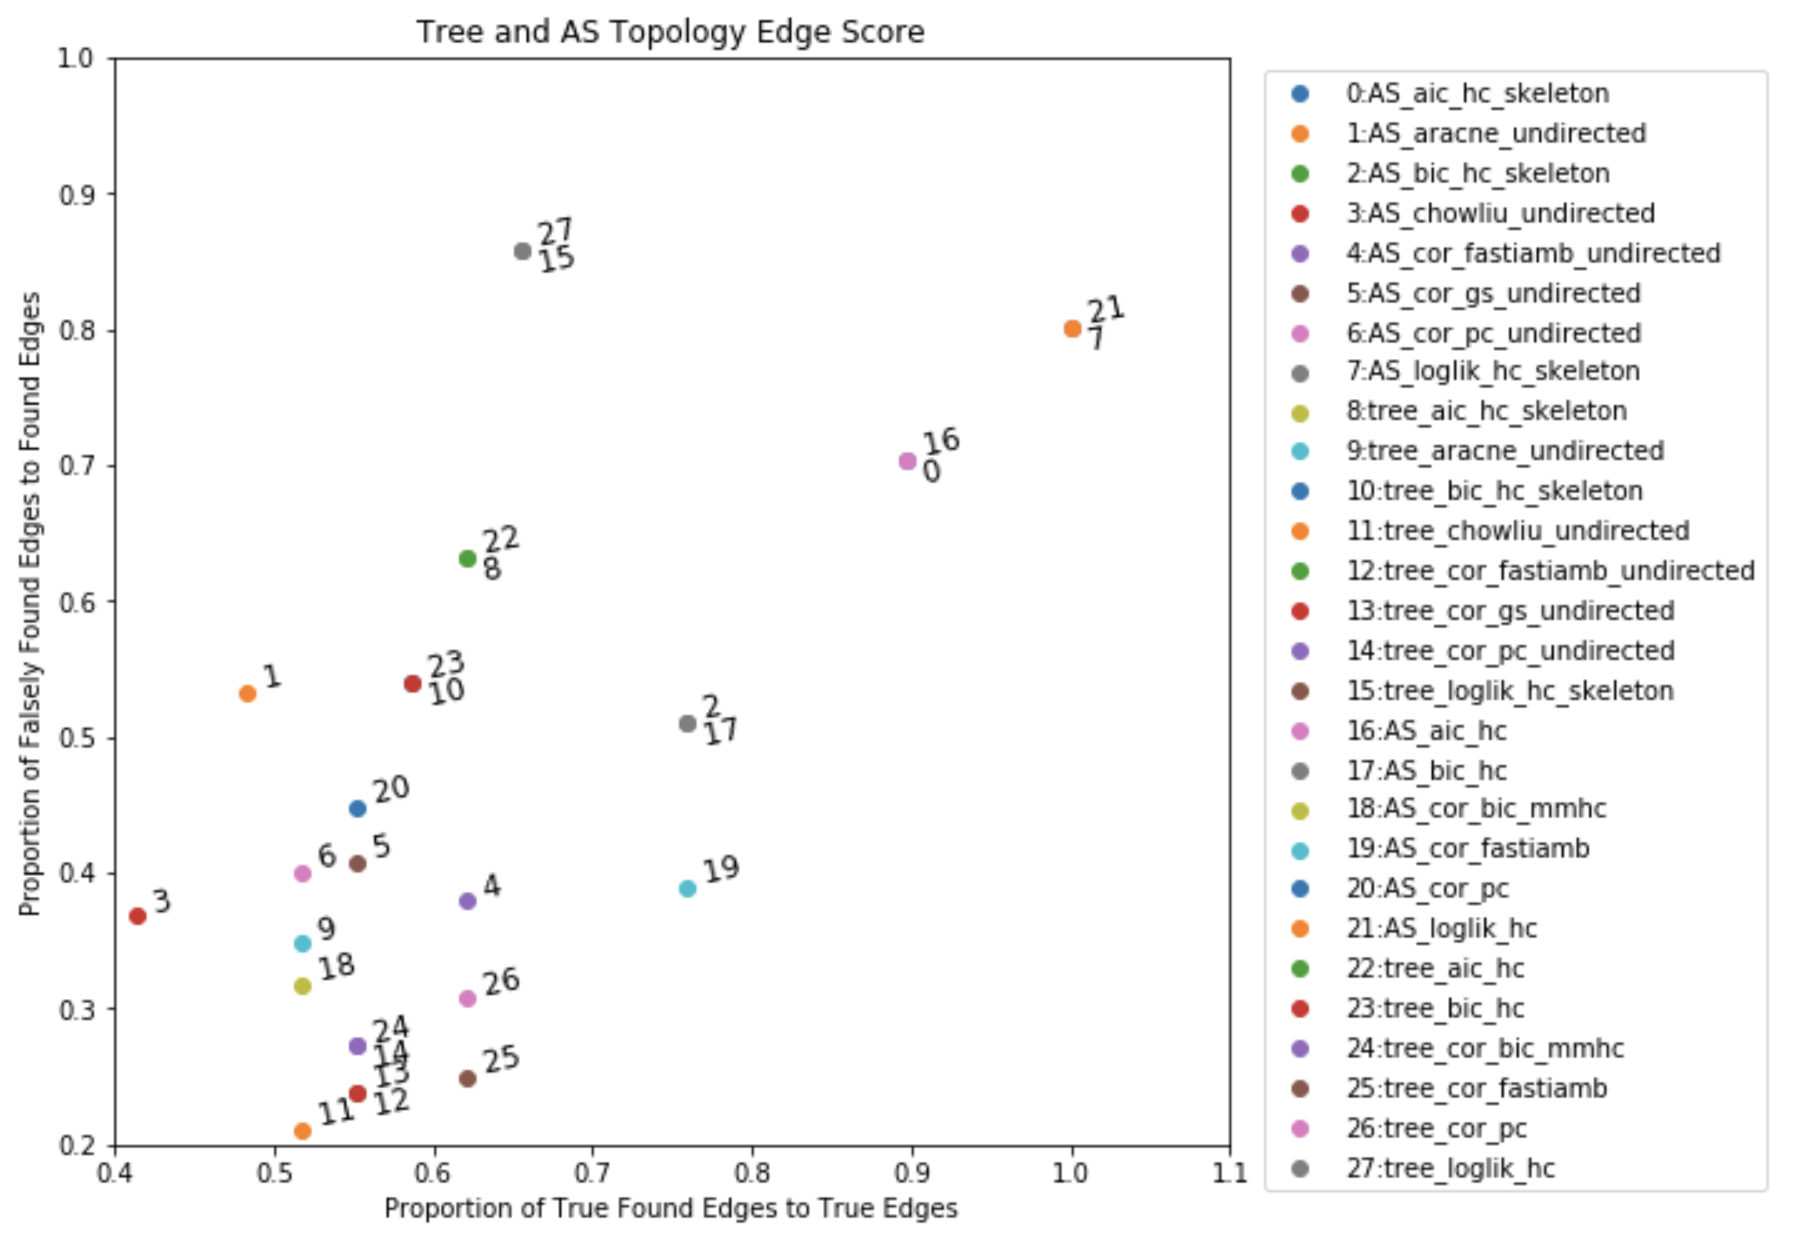
\includegraphics[height=8cm]{images/edge_scores.png}
    \caption{Scatter plot of the proportion of edges found in the directed acyclic graph (DAG) that are true to the connectivity in the network resembling the topology of internet autonomous systems (AS) or of a random tree (relative to all possible edges in the true topology) versus the proportion of edges found the DAG that are not in the connectivity of the true topology (relative to all edges in the DAG).
}
\label{fig:edges}
\end{figure}
\begin{figure}%
    \centering
    \subfloat{{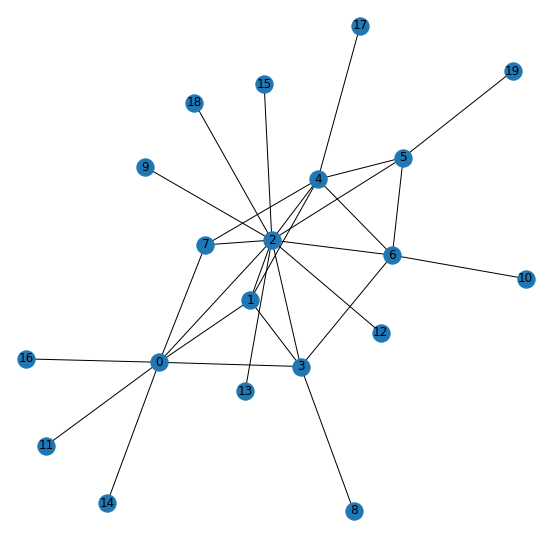
\includegraphics[width=3cm]{images/AS_graph_random_delay_200days_equalbias.png} }}%
    \qquad
    \subfloat{{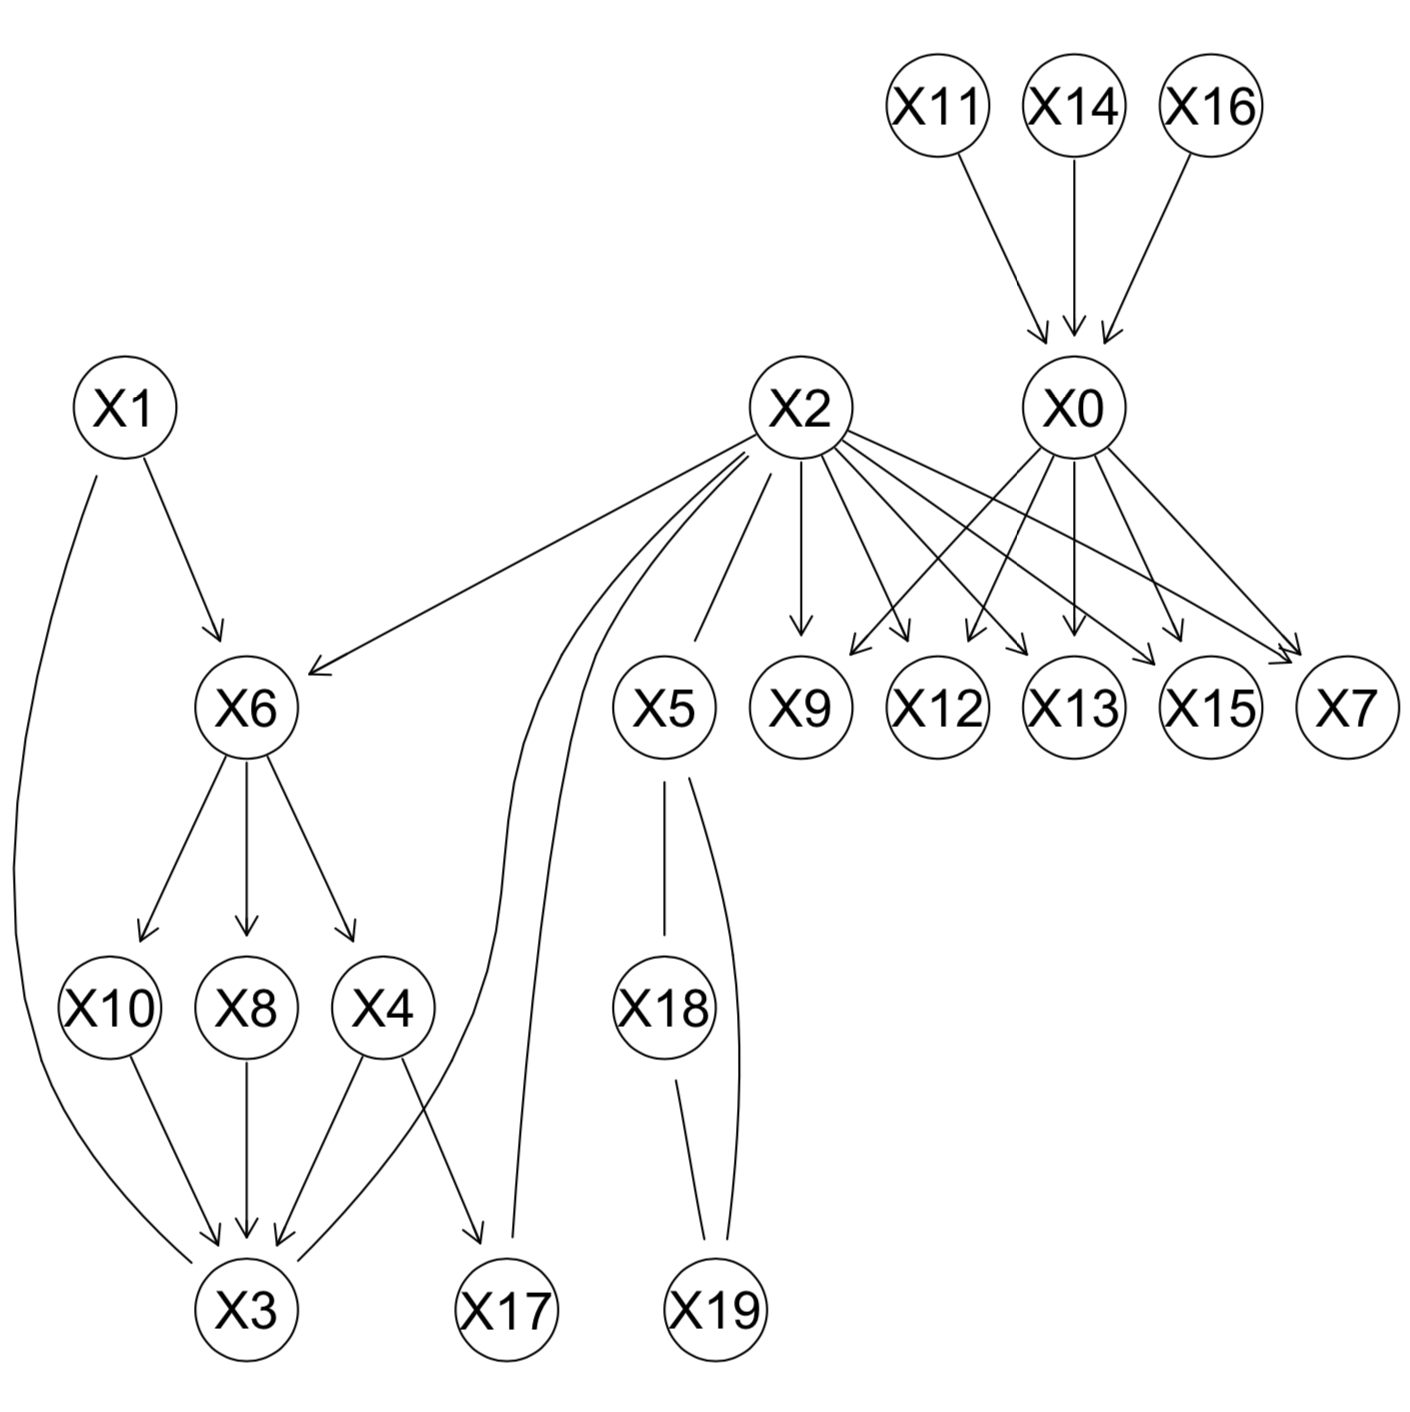
\includegraphics[width=3cm]{images/AS_fastiamb.png} }}%
    \caption{Real connectivity topology resembling the internet autonomous system network (left) versus directed acyclic graph (DAG) learned by the incremental association Markov blanket (IAMB) algorithm on the router packet counts with simulated traffic routed according to Dijkstra's shortest path (right). The proportion of true found edges to total true edges for this topology learned by the IAMB algorithm is 0.76, while the proportion of falsely found edges to total found edges is 0.39.
}%
    \label{fig:AS}%
\end{figure}
\begin{figure}%
    \centering
    \subfloat{{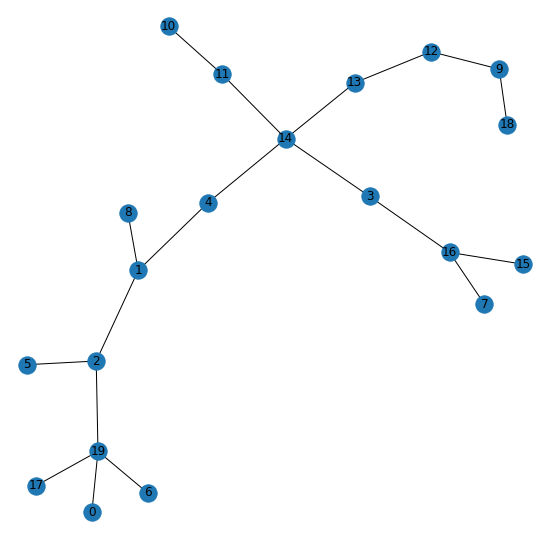
\includegraphics[width=3cm]{images/tree_graph_random_delay_200days_equalbias.png} }}%
    \qquad
    \subfloat{{\includegraphics[width=3cm]{images/tree_fastiamb.png} }}%
    \caption{ Real connectivity topology resembling a tree network (left) versus directed acyclic graph (DAG) learned by the incremental association Markov blanket (IAMB) algorithm on the router packet counts with simulated traffic routed according to Dijkstra's shortest path (right). The proportion of true found edges to total true edges for this topology learned by the IAMB algorithm is 0.62, while the proportion of falsely found edges to total found edges is 0.25.}%
    \label{fig:tree}%
\end{figure}

In the learned DAGs (Figure \ref{fig:AS}; Figure \ref{fig:tree}), the edges represent conditional dependence between nodes. As described previously, a directed edge from A to B means that B is conditionally independent of all other nodes in the graph (except for any children nodes it has) given A. Therefore, the direction of the edge represents the direction of traffic flow. However, if the values of A are independent of all other nodes in the graph (save its children) given B and the values of B are independent of all other nodes in the graph (save its children) given A, then the IAMB algorithm is unable to determine the direction of the indication relationship and the edge is left undirected. We observe in general that for either the AS or tree topologies, the source nodes are closer to the root of the DAG (having fewer parents) compared to the destination nodes (i.e., X18 and X19).

All code for generating the simulated topologies, network traffic and DAGs as well as for comparing the learned DAGs to the real topologies is available \href{https://github.com/fizzX/cs143-final}{here}.


\section{Conclusion}

From this work we learned that DAG structure learning can generally be used to reveal network traffic patterns for AS and tree topologies. To the best of our knowledge, this is the first study to compare DAG structure learning algorithms to recover network traffic flows aggregated on the host level. With simulation data where the networks have 20 nodes and 200 samples ("days") of activity and routing is done using a link state scheme with Dijkstra's shortest path algorithm, the IAMB algorithm recovers the highest rate of true edges in the DAG compared to the ground truth topology. This project contributes to the literature the observation that DAG structure learning can be used to resemble network traffic flow patterns based only on packet counts at routers. The project was a strong success because we showed that there is an algorithm that can recover far more true edges in the DAG relative to the real topology connectivity compared to extraneous edges (edges in DAG that are not shown in the real connectivity).

Our immediate next step would be to run simulations with different numbers of pings per day and different numbers of days. This would allow us to determine how robust our current findings are to sample size, which would be useful since allowing smaller sample sizes for the number of pings per "day” would allow us to use this method to learn traffic flow patterns over shorter time intervals (if we measured packet counts at routers not for a full day but instead for half of a day or even just an hour). Since the traffic flow topologies are inherently dynamic (with network traffic changing over time), learning DAGs accurately with data from shorter time intervals (instead of a full day) would be useful for finer mapping of the traffic flows.

In the future, we would also run more simulations on different types of network topology archetypes modeled after actual content delivery networks and other types of internet service networks. The AS and tree topologies are certainly not the only topologies in LANs. Additionally, we hope to find real-world internet traffic data for network topologies that we can observe. Although we did find a real-world dataset from CAIDA along with other maps of router connectivity, we were unable to discover the actual network topology that the dataset was derived from and therefore we would have had no way to evaluate whether the learned DAG was representative of the true topology.

A long-term goal would be to investigate whether other graphical models as opposed to DAGs can be used to reveal network traffic among hosts. Specifically, we could investigate how machine learning approaches such as those used for graphical neural networks could be applied to learn traffic flow patterns based only on router packet counts.


\begin{thebibliography}{00}
\bibitem{b1} Iliofotou, M., Pappu, P., Faloutsos, M., Mitzenmacher, M., Singh, S., \& Varghese, G. (2007). ``Network monitoring using traffic dispersion graphs (tdgs)''. Proceedings of the 7th ACM SIGCOMM Conference on Internet Measurement, 315-320.
\bibitem{b2} Cisco. ``Introduction to the Cisco TOP NetFlow''. May 2012.
\bibitem{b3} Donnet, B., \& Longstaff, I. (2007). ``Combining MIMO Radar with OFDM Communications''. 2006 European Radar Conference, 37-40.
\bibitem{b4} Markus Kalisch, Martin Machler, Diego Colombo, Marloes H. Maathuis, \& Peter Buhlmann. (2012). ``Causal Inference Using Graphical Models with the R Package pcalg''. Journal of Statistical Software, 47(11), 1-26.
\bibitem{b5} Hausman, D., \& Woodward, J. (1999). ``Independence, invariance and the causal Markov condition''. The British Journal for the Philosophy of Science, 50(4), 521-583.
\bibitem{b6} White, A., \& Vignes, M. (2018). ``Causal Queries from Observational Data in Biological Systems via Bayesian Networks: An Empirical Study in Small Networks''. ArXiv.org, ArXiv.org, May 4, 2018.
\bibitem{b7} Nandy, P., Hauser, A., \& Maathuis, M. (2018). High-dimensional consistency in score-based and hybrid structure learning. Annals of Statistics, 46(6A), 3151-3183.
\bibitem{b8} Spirtes, P., Glymour, C., \& Scheines, R. (2000). Causation, prediction, and search / Peter Spirtes, Clark Glymour, and Richard Scheines ; with additional material by David Heckerman ... [et al.] (2nd ed., Adaptive computation and machine learning). Cambridge, Mass.: MIT Press.
\bibitem{b9} Tsamardinos, Ioannis \& Aliferis, Constantin \& Statnikov, Alexander. (2003). Algorithms for Large Scale Markov Blanket Discovery. Proceedings of the sixteenth international Florida artificial intelligence research society conference. 376-381.
\bibitem{b10} Scutari, M., Graafland, C., \& Gutiérrez, J. (2018). Who Learns Better Bayesian Network Structures: Accuracy and Speed of Structure Learning Algorithms. Journal of Machine Learning Research (72, Proceedings Track, PGM 2018), 416-427; extended version in International Journal of Approximate Reasoning, 115:235-253.
\bibitem{b11} Aric A. Hagberg, Daniel A. Schult and Pieter J. Swart, "Exploring network structure, dynamics, and function using NetworkX”, in Proceedings of the 7th Python in Science Conference (SciPy2008), Gäel Varoquaux, Travis Vaught, and Jarrod Millman (Eds), (Pasadena, CA USA), pp. 11–15, Aug 2008
\bibitem{b12} Elmokashfi, A. Kvalbein and C. Dovrolis, "On the Scalability of BGP: The Role of Topology Growth,” in IEEE Journal on Selected Areas in Communications, vol. 28, no. 8, pp. 1250-1261, October 2010.
\bibitem{b13} Wang, Xiaodong, Lei Wang, and Yingjie Wu. "An optimal algorithm for Prufer codes.” Journal of Software Engineering and Applications 2.02 (2009): 111.
\bibitem{b14} Magoni, D., \& Pansiot, J. (2001). Analysis of the Autonomous System network topology. Acm Sigcomm Computer Communication Review, 31(3), 26-37.
\bibitem{b15} Marco Scutari (2010). Learning Bayesian Networks with the bnlearn R Package. Journal of Statistical Software, 35(3), 1-22.
\bibitem{b16} R Core Team (2017). R: A language and environment for statistical computing. R Foundation for Statistical Computing, Vienna, Austria.

\end{thebibliography}

\end{document}
